\definecolor{qqqqcc}{rgb}{0,0,0.8}
\definecolor{qqqqzz}{rgb}{0,0,0.6}
\definecolor{ccqqqq}{rgb}{0.8,0,0}
\definecolor{wwwwww}{rgb}{0.4,0.4,0.4}

\begin{subfigure}{0.4\textwidth}
    \centering
    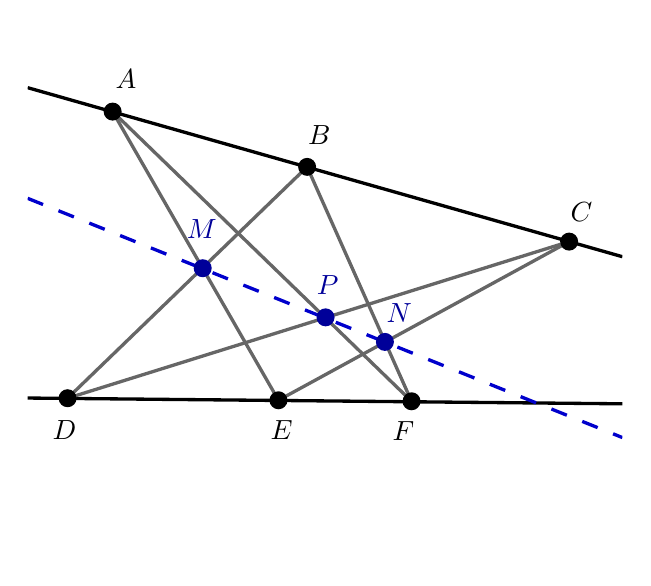
\begin{tikzpicture}[scale = 1.3]
        \clip(-3.03,0.22) rectangle (2.78,5.4);
        \draw [line width=1.2pt,domain=-3.03:2.78] plot(\x,{(--7.51-0.54*\x)/1.9});
        \draw [line width=1.2pt,domain=-3.03:2.78] plot(\x,{(--3.61-0.02*\x)/2.06});
        \draw [line width=1.2pt,color=wwwwww] (-2.2,4.58)-- (-0.58,1.76);
        \draw [line width=1.2pt,color=wwwwww] (-2.2,4.58)-- (0.72,1.75);
        \draw [line width=1.2pt,color=wwwwww] (-2.64,1.78)-- (-0.3,4.04);
        \draw [line width=1.2pt,color=wwwwww] (-2.64,1.78)-- (2.26,3.31);
        \draw [line width=1.2pt,color=wwwwww] (-0.58,1.76)-- (2.26,3.31);
        \draw [line width=1.2pt,color=wwwwww] (-0.3,4.04)-- (0.72,1.75);
        \draw [line width=1.2pt,dash pattern=on 6pt off 6pt,color=qqqqcc,domain=-3.03:2.78] plot(\x,{(--4.5-0.72*\x)/1.79});
        \begin{scriptsize}
            \normalsize
            \fill [color=black] (-2.2,4.58) circle (2.5pt);
            \draw[color=black] (-2.07,4.9) node {$A$};
            \fill [color=black] (-0.3,4.04) circle (2.5pt);
            \draw[color=black] (-0.18,4.35) node {$B$};
            \fill [color=black] (2.26,3.31) circle (2.5pt);
            \draw[color=black] (2.38,3.6) node {$C$};
            \fill [color=black] (-2.64,1.78) circle (2.5pt);
            \draw[color=black] (-2.67,1.47) node {$D$};
            \fill [color=black] (-0.58,1.76) circle (2.5pt);
            \draw[color=black] (-0.55,1.47) node {$E$};
            \fill [color=black] (0.72,1.75) circle (2.5pt);
            \draw[color=black] (0.64,1.46) node {$F$};
            \fill [color=qqqqzz] (-1.32,3.05) circle (2.5pt);
            \draw[color=qqqqzz] (-1.33,3.43) node {$M$};
            \fill [color=qqqqzz] (-0.12,2.57) circle (2.5pt);
            \draw[color=qqqqzz] (-0.1,2.89) node {$P$};
            \fill [color=qqqqzz] (0.46,2.33) circle (2.5pt);
            \draw[color=qqqqzz] (0.6,2.61) node {$N$};
        \end{scriptsize}
    \end{tikzpicture}
    \caption{Transversal $M-P-N$.}
\end{subfigure}
\hspace{0.1\textwidth}
\begin{subfigure}{0.4\textwidth}
    \centering
    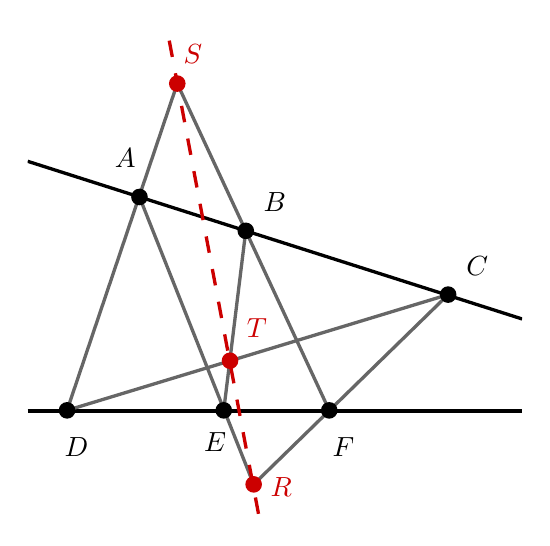
\begin{tikzpicture}[scale = 1]
        \clip(-3.01,-7.4) rectangle (3.27,-1.18);
        \draw [line width=1.2pt,domain=-3.01:3.27] plot(\x,{(-15.04-1.25*\x)/3.92});
        \draw [line width=1.2pt,domain=-3.01:3.27] plot(\x,{(-20.14-0*\x)/3.33});
        \draw [line width=1.2pt,color=wwwwww] (-1.11,-1.89)-- (-2.51,-6.04);
        \draw [line width=1.2pt,color=wwwwww] (-1.11,-1.89)-- (0.82,-6.04);
        \draw [line width=1.2pt,color=wwwwww] (-0.14,-6.98)-- (-1.59,-3.33);
        \draw [line width=1.2pt,color=wwwwww] (2.33,-4.57)-- (-0.14,-6.98);
        \draw [line width=1.2pt,color=wwwwww] (-0.52,-6.04)-- (-0.24,-3.76);
        \draw [line width=1.2pt,color=wwwwww] (-2.51,-6.04)-- (2.33,-4.57);
        \draw [line width=1.2pt,dash pattern=on 6pt off 6pt,color=ccqqqq,domain=-3.01:3.27] plot(\x,{(-7.46-5.09*\x)/0.96});
        \begin{scriptsize}
            \normalsize
            \fill [color=black] (-1.59,-3.33) circle (3pt);
            \draw[color=black] (-1.77,-2.83) node {$A$};
            \fill [color=black] (-0.24,-3.76) circle (3.0pt);
            \draw[color=black] (0.13,-3.4) node {$B$};
            \fill [color=black] (2.33,-4.57) circle (3.0pt);
            \draw[color=black] (2.7,-4.21) node {$C$};
            \fill [color=black] (-2.51,-6.04) circle (3.0pt);
            \draw[color=black] (-2.39,-6.51) node {$D$};
            \fill [color=black] (-0.52,-6.04) circle (3.0pt);
            \draw[color=black] (-0.63,-6.44) node {$E$};
            \fill [color=black] (0.82,-6.04) circle (3.0pt);
            \draw[color=black] (1,-6.51) node {$F$};
            \fill [color=ccqqqq] (-1.11,-1.89) circle (3.0pt);
            \draw[color=ccqqqq] (-0.91,-1.52) node {$S$};
            \fill [color=ccqqqq] (-0.14,-6.98) circle (3.0pt);
            \draw[color=ccqqqq] (0.21,-7.01) node {$R$};
            \fill [color=ccqqqq] (-0.44,-5.41) circle (3.0pt);
            \draw[color=ccqqqq] (-0.1,-5) node {$T$};
        \end{scriptsize}
    \end{tikzpicture}
    \caption{Transversal $S-T-R$.}
\end{subfigure}